\begin{enumerate}
\item Inicio de sesi'on: \newline
Cuando un m'edico enciende su PDA para empezar a trabajar, lo primero que se encuentra es con la pantalla Inicio de sesi'on. El m'edico deber'a introducir su nombre de usuario y su clave personal en los cuadros de texto correspondientes vali'endose del teclado del PDA y pulsar el bot'on Aceptar. Este es un procedimiento rutinario que impide que personal no autorizado pueda acceder a informaci'on confidencial del hospital.

\begin{figure*}[h!]
	\begin{center}
        		\framebox{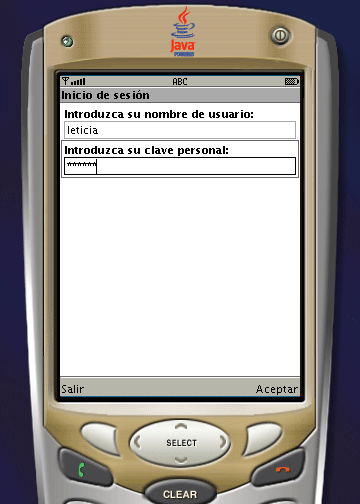
\includegraphics[scale=0.5]{inicio.png}}
     	\end{center}
    	\caption{Diagrama de secuencia del inicio de sesi'on}\label{fig:inicio_sesion}
\end{figure*}

En caso de que el m'edico no haya introducido correctamente su nombre de usuario o su clave personal, no podr'a acceder a la aplicaci'on. Se le informar'a de ello y se le dar'a la oportunidad de introducir sus datos de nuevo.

\begin{figure*}[h!]
	\begin{center}
        		\framebox{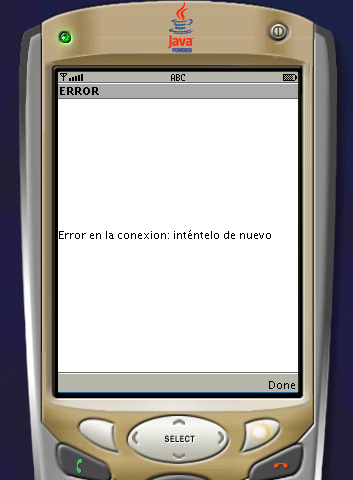
\includegraphics[scale=0.5]{error_inicio.png}}
     	\end{center}
    	\caption{Pantalla de error en el inicio de sesi'on}\label{fig:pantalla_error_inicio}
\end{figure*}

En caso de que puls'aramos el bot'on Salir, en el margen inferior izquierdo de la pantalla, saldr'iamos de la aplicaci'on y se apagar'ia el PDA.

\item Men'u principal:\newline
Una vez iniciada la sesi'on, el m'edico tiene acceso al men'u principal donde se le ofertan todas las utilidades de la aplicaci'on.

\begin{figure*}[h!]
	\begin{center}
        		\framebox{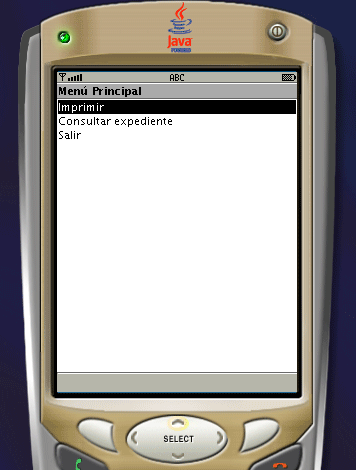
\includegraphics[scale=0.5]{menu_principal.png}}
     	\end{center}
    	\caption{Pantalla del men'u principal}\label{fig:pantalla_principal}
\end{figure*}

Para elegir una opci'on del men'u debe desplazarse por el men'u con las flechas centrales hacia arriba y hacia abajo y pulsar Select cuando tenga seleccionada la tarea que desea realizar.

Ahora hablaremos de las diferentes opciones del men'u principal:
\begin{itemize}

\item Men'u de impresi'on:\newline
A trav'es de esta opci'on podemos imprimir un documento disponible del paciente del hospital deseado: s'olo tenemos que elegir el tipo de documento a imprimir (Expediente o 'Ultimos an'alisis) e introducir a trav'es del teclado el nombre del paciente del que precisamos los documentos. Una vez introducidos estos datos, solo hay que pulsar el bot'on Aceptar, en el margen inferior derecho de la pantalla.

\begin{figure*}[h!]
	\begin{center}
        		\framebox{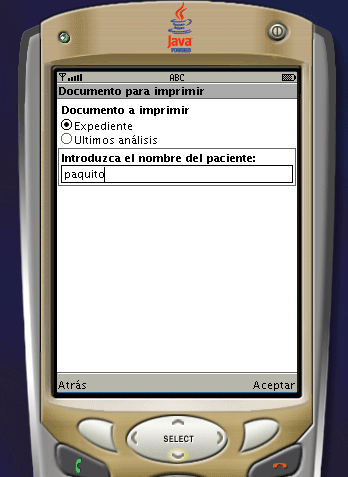
\includegraphics[scale=0.5]{menu_imprimir.png}}
     	\end{center}
   	\caption{Pantalla del men'u de impresi'on}\label{fig:pantalla_imprimir}
\end{figure*}

El bot'on Atr'as nos devuelve al men'u principal.

En caso de que introduzcamos mal el nombre del paciente, no est'en disponibles los documentos o no sea posible el uso de las impresoras, se informar'a al usuario y se le instar'a a intentarlo m'as tarde.

\begin{figure*}[h!]
	\begin{center}
        		\framebox{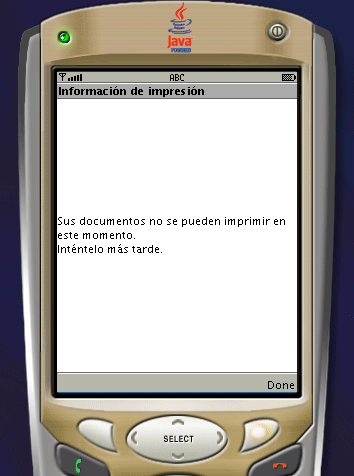
\includegraphics[scale=0.5]{error_imprimir.png}}
     	\end{center}
    	\caption{Pantalla de error en el procedimiento de imprimir}\label{fig:error_imprimir}
\end{figure*}

En caso de que no haya ning'un problema en la realizaci'on  de la tarea, se informar'a al usuario de la impresora por la que se llevar'a a cabo la impresi'on solicitada.

\begin{figure*}[h!]
	\begin{center}
        		\framebox{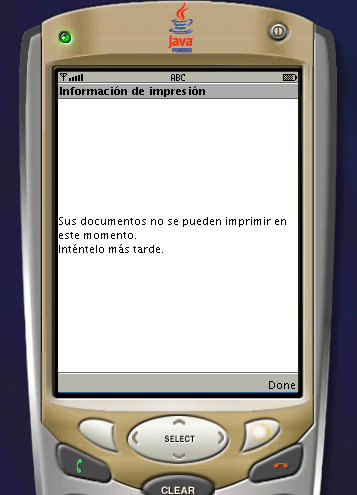
\includegraphics[scale=0.5]{acierto_imprimir.png}}
     	\end{center}
    	\caption{Pantalla de informaci'on de impresi'on}\label{fig:acierto_imprimir}
\end{figure*}

\item Consultar expediente:\newline
Con esta opci'on podemos visualizar en la pantalla del PDA el expediente del paciente deseado. Al seleccionarla llegamos a  una pantalla en la solo tenemos que introducir el nombre del paciente y pulsar el bot'on Aceptar para acceder al expediente deseado.

\begin{figure*}[h!]
	\begin{center}
        		\framebox{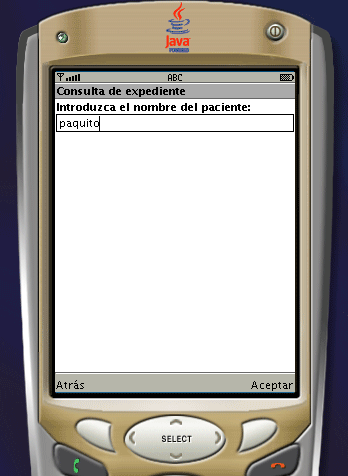
\includegraphics[scale=0.5]{menu_consulta.png}}
     	\end{center}
    	\caption{Pantalla de petici'on de consulta de expediente}\label{fig:menu_consulta}
\end{figure*}

El bot'on Atr'as nos devuelve al men'u principal.

En caso de que introduzcamos mal el nombre del paciente o no est'en disponibles los documentos, se informar'a al usuario.

\begin{figure*}[h!]
	\begin{center}
        		\framebox{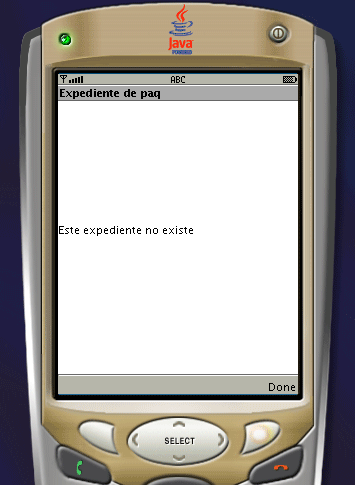
\includegraphics[scale=0.5]{error_consulta.png}}
     	\end{center}
    	\caption{Pantalla de error en la consulta de expediente}\label{fig:error_consulta}
\end{figure*}

En caso de que los datos sean correctos se mostrar'a por pantalla el expediente del paciente solicitado.

%falta pantallazo de esto!!!!!!!!!!!!!!!!!!!!!!!!!!!!!

\item Salir:\newline
Esta opci'on nos permite salir de la aplicaci'on y apagar el PDA.
 
\end{itemize}


\end{enumerate}